\chapter{Search for Resonant Di-Higgs }
\label{ch:diHiggs_search}
\section{Introduction and Motivation}
The study of Higgs boson pair production provides a unique opportunity to probe the Higgs self-coupling and to search for physics
beyond the Standard Model (BSM). In the SM, Higgs boson pairs are dominantly produced via gluon-gluon fusion (ggF) through triangle
and box diagrams, as shown in Fig.~\ref{SMLO_ggHH_production}, that exhibit destructive interference.
The predicted cross section for non-resonant di-Higgs production is small, \(0.01449 \pm 0.000019\)~pb,
making this process challenging to observe.
\begin{figure}[!htbp]
    \begin{center}
        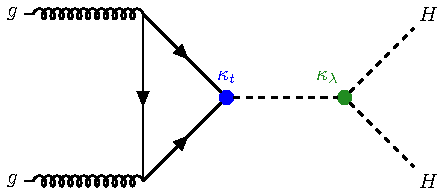
\includegraphics[width=0.45\textwidth]{figures/diHiggsSearches/fey_HH_Triangle.pdf} %
        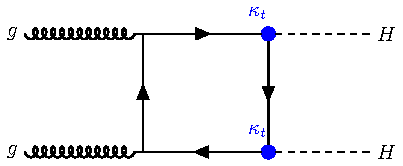
\includegraphics[width=0.45\textwidth]{figures/diHiggsSearches/fey_HH_Box.pdf}
    \end{center}
    \caption{Feynman diagrams for leading-order Higgs boson pair production via gluon fusion}
    \label{SMLO_ggHH_production}
\end{figure}
\begin{figure}[!htbp]
    \begin{center}
        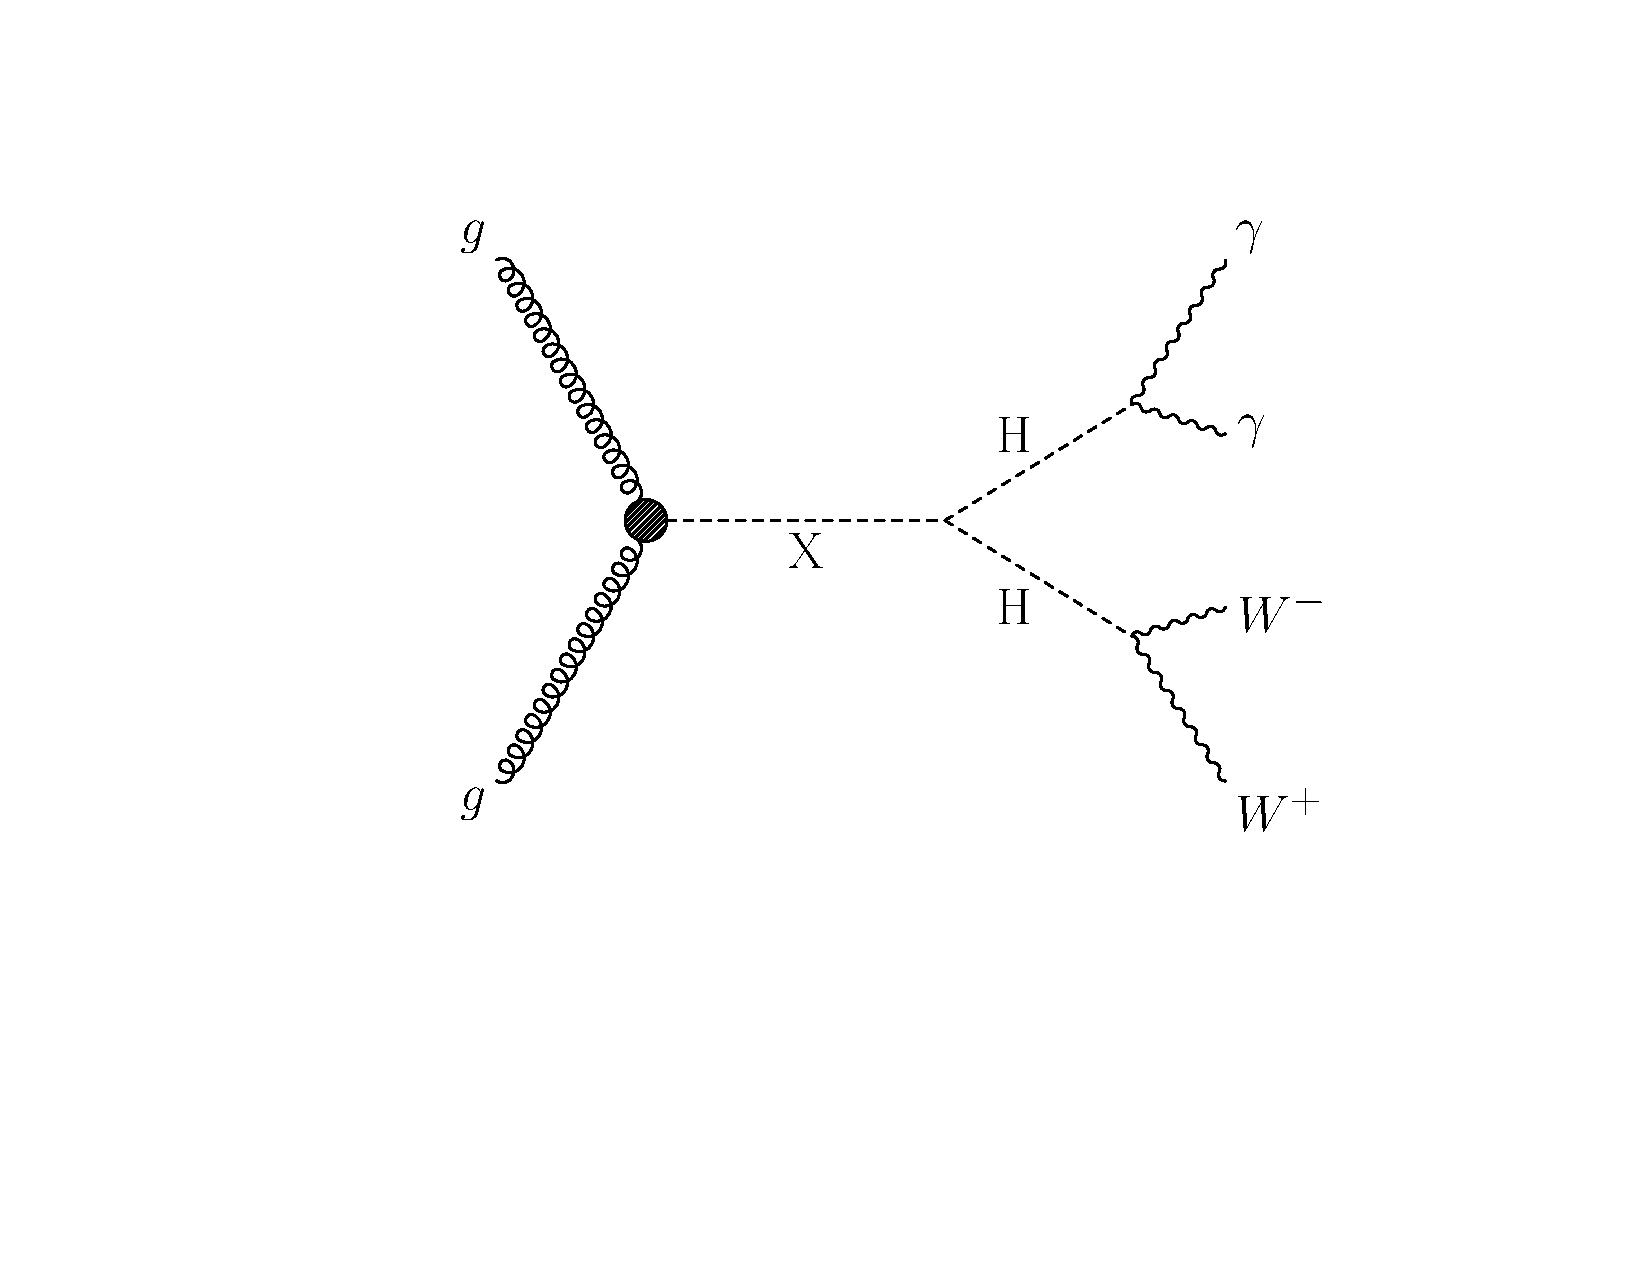
\includegraphics[width=0.45\textwidth]{figures/diHiggsSearches/fey_XHH_HHWWgg.pdf}
    \end{center}
    \caption{Feynman diagram for resonant di-Higgs production in the \HH channel}
    \label{XHHFeynmanDiagram}
\end{figure}


Extensions of the SM, such as the Next-to-Minimal Supersymmetric Standard Model (NMSSM), Randall-Sundrum models, or the two-Higgs
doublet model (2HDM), predict resonant di-Higgs production. In these scenarios, a heavy resonance \(X\) decays into two Higgs
bosons, which subsequently decay into \(WW\) and \(\gamma\gamma\), as shown in Fig.~\ref{XHHFeynmanDiagram}.

This analysis specifically targets the \HHWW channel, utilizing the clean diphoton final state to maximize sensitivity while accounting for all possible jet topologies.
Although this channel has a relatively low branching fraction, as shown in Fig.~\ref{fig:HH_BF},
it provides a distinctive signature for Beyond Standard Model (BSM) searches due to
the presence of a clean diphoton final state combined with couplings to vector bosons.

\begin{figure}[!htbp]
    \centering
    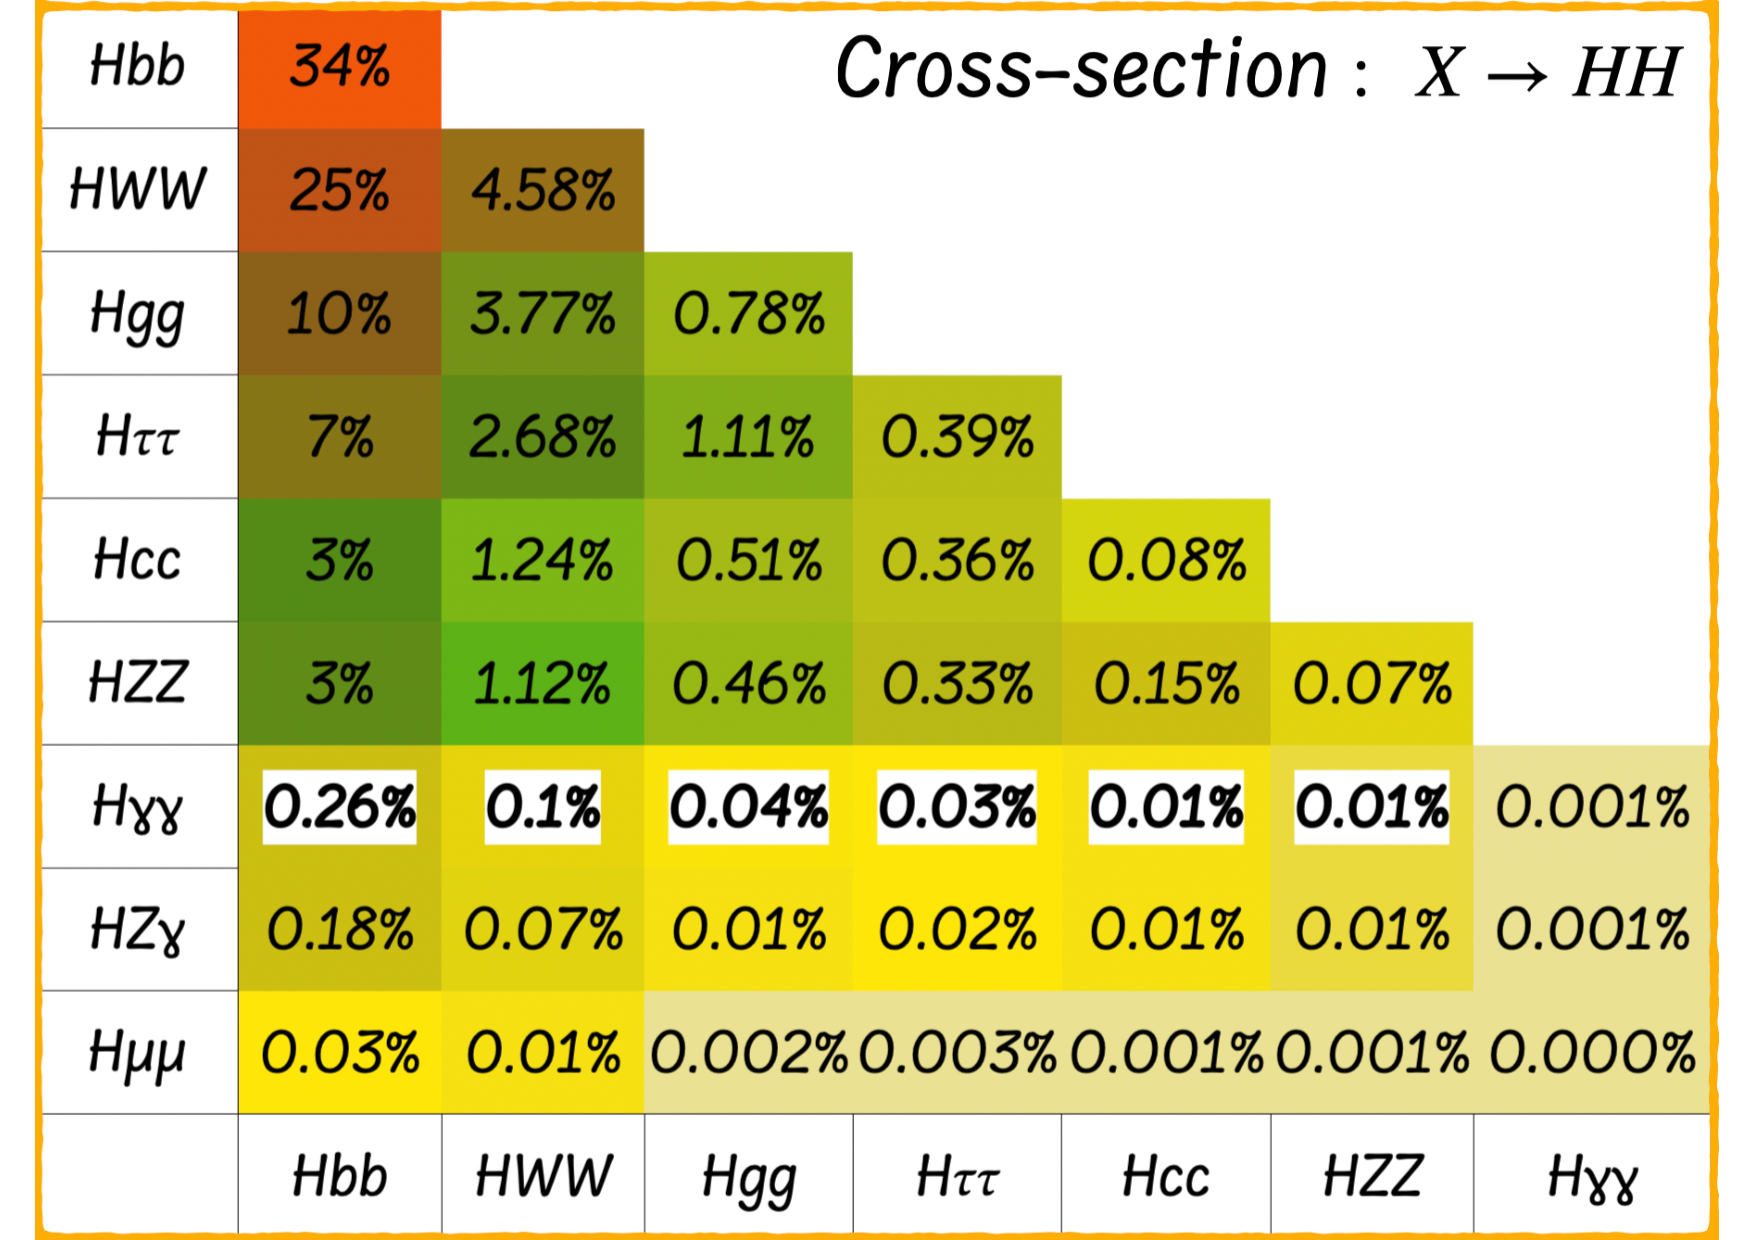
\includegraphics[width=0.95\textwidth]{figures/diHiggsSearches/HH_BF.pdf}
    \caption{Branching fractions of Higgs boson decays.}
    \label{fig:HH_BF}
\end{figure}


\section{Analysis Overview}
The analysis is performed using the full Run-2 Ultra-Legacy dataset, corresponding to an integrated luminosity of 138~fb\(^{-1}\) at
\(\sqrt{s} = 13\)~TeV. The following decay channels are explored:
\begin{itemize}
    \item \textbf{Semi-leptonic (\(l\nu qq\gamma\gamma\)):} One \(W\) boson decays leptonically (\(W \to l\nu\)), and the other
    decays hadronically (\(W \to qq\)).
    \item \textbf{Fully hadronic (\(4q\gamma\gamma\)):} Both \(W\) bosons decay hadronically (\(W \to qq\)).
\end{itemize}

\section{Unique Features of the Analysis}
This analysis incorporates several innovative aspects, as detailed below:

\begin{itemize}
    \item \textbf{Comprehensive Topology Coverage:}
    For the first time, all jet topologies are tagged within a single analysis. These include boosted, semi-boosted, resolved, and scenarios where leptons are reconstructed inside jets.

    \item \textbf{Signal Definition:}
    The signal is defined as the sum of three di-Higgs decay possibilities:
    \[
    HH \to WW\gamma\gamma + ZZ\gamma\gamma + bb\gamma\gamma.
    \]
    Since the hadronic decay topologies are similar for all three channels, it is challenging to reduce contamination from the \(ZZ\gamma\gamma\) and \(bb\gamma\gamma\) channels in our primary signal of interest, \(WW\gamma\gamma\). The signal definition is further refined with the following considerations:
    \begin{itemize}
        \item The analysis is optimized for the \(HH \to WW\gamma\gamma\) channel.
        \item For \(HH \to WW\gamma\gamma\), two decay modes of the \(W\)-bosons are considered: fully hadronic and semi-leptonic. The analysis optimization is performed based on these two final states.
        \item For \(HH \to ZZ\gamma\gamma\), due to the low branching fraction and negligible semi-leptonic contribution, the semi-leptonic decay mode is excluded from the analysis.
        \item The \(bb\gamma\gamma\) channel is included after applying a b-jet veto. This serves multiple purposes:
        \begin{enumerate}
            \item It reduces the contribution from the \(bb\gamma\gamma\) channel, ensuring that the limit is primarily driven by the \(WW\gamma\gamma\) channel rather than \(bb\gamma\gamma\).
            \item It makes the analysis orthogonal to the \(HH \to bb\gamma\gamma\) analysis.
            \item Events rejected by the \(HH \to bb\gamma\gamma\) analysis are exploited, thereby utilizing additional information from the same dataset.
            \item The b-jet veto also rejects events from \(HH \to ZZ\gamma\gamma\) where the \(Z\)-bosons decay into b-quarks.
        \end{enumerate}
    \end{itemize}

    \item \textbf{Mass Ranges:}
    The resonance \(X\) is studied over a mass range of 250~GeV to 3000~GeV.

    \item \textbf{Leptons Inside Jets:}
    Events where leptons are reconstructed within jets are included, thereby enhancing sensitivity to specific Beyond Standard Model (BSM) scenarios.
\end{itemize}

\section{Event Selection}


The event selection optimizes sensitivity to semi-leptonic and fully hadronic channels, with the following criteria:

\subsection*{Photon Selection}
\begin{itemize}
    \item A boosted decision tree (BDT) classifier is trained to separate photons from jets~\cite{Sirunyan:2018ouh}.
            The output of this BDT is referred to as the photon ID score
            \footnote{For the boosted regime, where the two photons are close by, the photon ID score was modified to
            account for reduced selection efficiency.
            This modified score is referred to as the ``modified photon ID," detailed in
            Appendix~\ref{appendix:ModifiedPhotonID}}. The photon $ID > -0.7$ is used as a preselection criterion.
    \item Leading photon \(p_T > 35\)~GeV and subleading photon \(p_T > 25\)~GeV.
    \item Photon transverse momentum fractions: \(p_T/m_{\gamma\gamma} > 0.33\) (leading) and \(> 0.25\) (subleading).
    \item Diphoton invariant mass requirement: \(100 < m_{\gamma\gamma} < 180\)~GeV.
\end{itemize}


\subsection*{Lepton Selection}
\begin{itemize}
    \item \textbf{Kinematics:} \(p_T > 10\)~GeV, \(|\eta| < 2.4\), and \(\Delta R(l, \gamma) > 0.4\).
    \item \textbf{\(Z\)-veto:} \(|m_{l\gamma} - 91.2| > 5\)~GeV to suppress contamination from \(Z\)-boson events.
    \item \textbf{ID requirements:}
        \begin{itemize}
            \item \textbf{For isolated electrons:} Use the isolated MVA ID with a signal efficiency of 80\%.
            \item \textbf{For isolated muons:} Require global muons with tight ID and an isolation threshold of 0.15.
            \item \textbf{For non-isolated electrons:} Use the non-isolated MVA ID with a signal efficiency of 80\%, ensuring \(\Delta R < 0.8\) with a good FatJet (as defined in the jet selection).
            \item \textbf{For non-isolated muons:} Require high \(p_T\) ID\todo[fancyline]{define High pT ID} without isolation criteria, ensuring \(\Delta R < 0.8\) with a good FatJet (as defined in the jet selection\todo[fancyline]{cite jet section}).
        \end{itemize}
\end{itemize}

\subsection*{Small Radius Jets (AK4 CHS)}
\begin{itemize}
    \item \textbf{ID:} Tight
    \item \textbf{PU Jet ID:} Tight
    \item \textbf{Kinematics:} \(p_T > 20\)~GeV, \(|\eta| < 2.4\)
    \item \textbf{Separation criteria:}
        \begin{itemize}
            \item \(\Delta R(\gamma, \text{jet}) > 0.4\)
            \item \(\Delta R(\text{Isolated Lepton, jet}) > 0.4\)
        \end{itemize}
\end{itemize}

\subsection*{FatJets (AK8 PUPPI)}
\begin{itemize}
    \item \textbf{Kinematics:} \(p_T > 100~\text{GeV}, |\eta| < 2.4\), with Tight Jet ID.
    \item \textbf{Separation criteria:}
    \begin{itemize}
        \item \(\Delta R(\gamma, \text{jet}) > 0.8\).
    \end{itemize}
    \item \textbf{Boosted \(H_{bb}\) jet veto:} \(X_{bb}/X_{\text{qcd}} < 0.9\).
    \item \textbf{Fully Hadronic Higgs Jet:}
    \begin{itemize}
        \item Particle Transformer\todo{define particle transformer in the footnote} Higgs Tagging score \(> 0.2\).
    \end{itemize}
    \item \textbf{Semi-Leptonic Higgs Jet:}
    \begin{itemize}
        \item \(\Delta R(\text{Non-isolated lepton}, \text{FatJet}) < 0.8\).
    \end{itemize}
    \item \textbf{Boosted \(W\)-Jet:}
    \begin{itemize}
        \item ParticleNet\todo{define particleNet in the footnote} loose working point for W-jet tagging.
        \item \(\Delta R(\text{Isolated leptons}, \text{FatJet}) > 0.8\).
    \end{itemize}
\end{itemize}

\subsection*{Event Selection}
The event selection is optimized for the semi-leptonic and fully hadronic channels and is summarized in Fig.~\ref{fig:event_selection_workflow}.
\begin{figure}[!htbp]
    \centering
    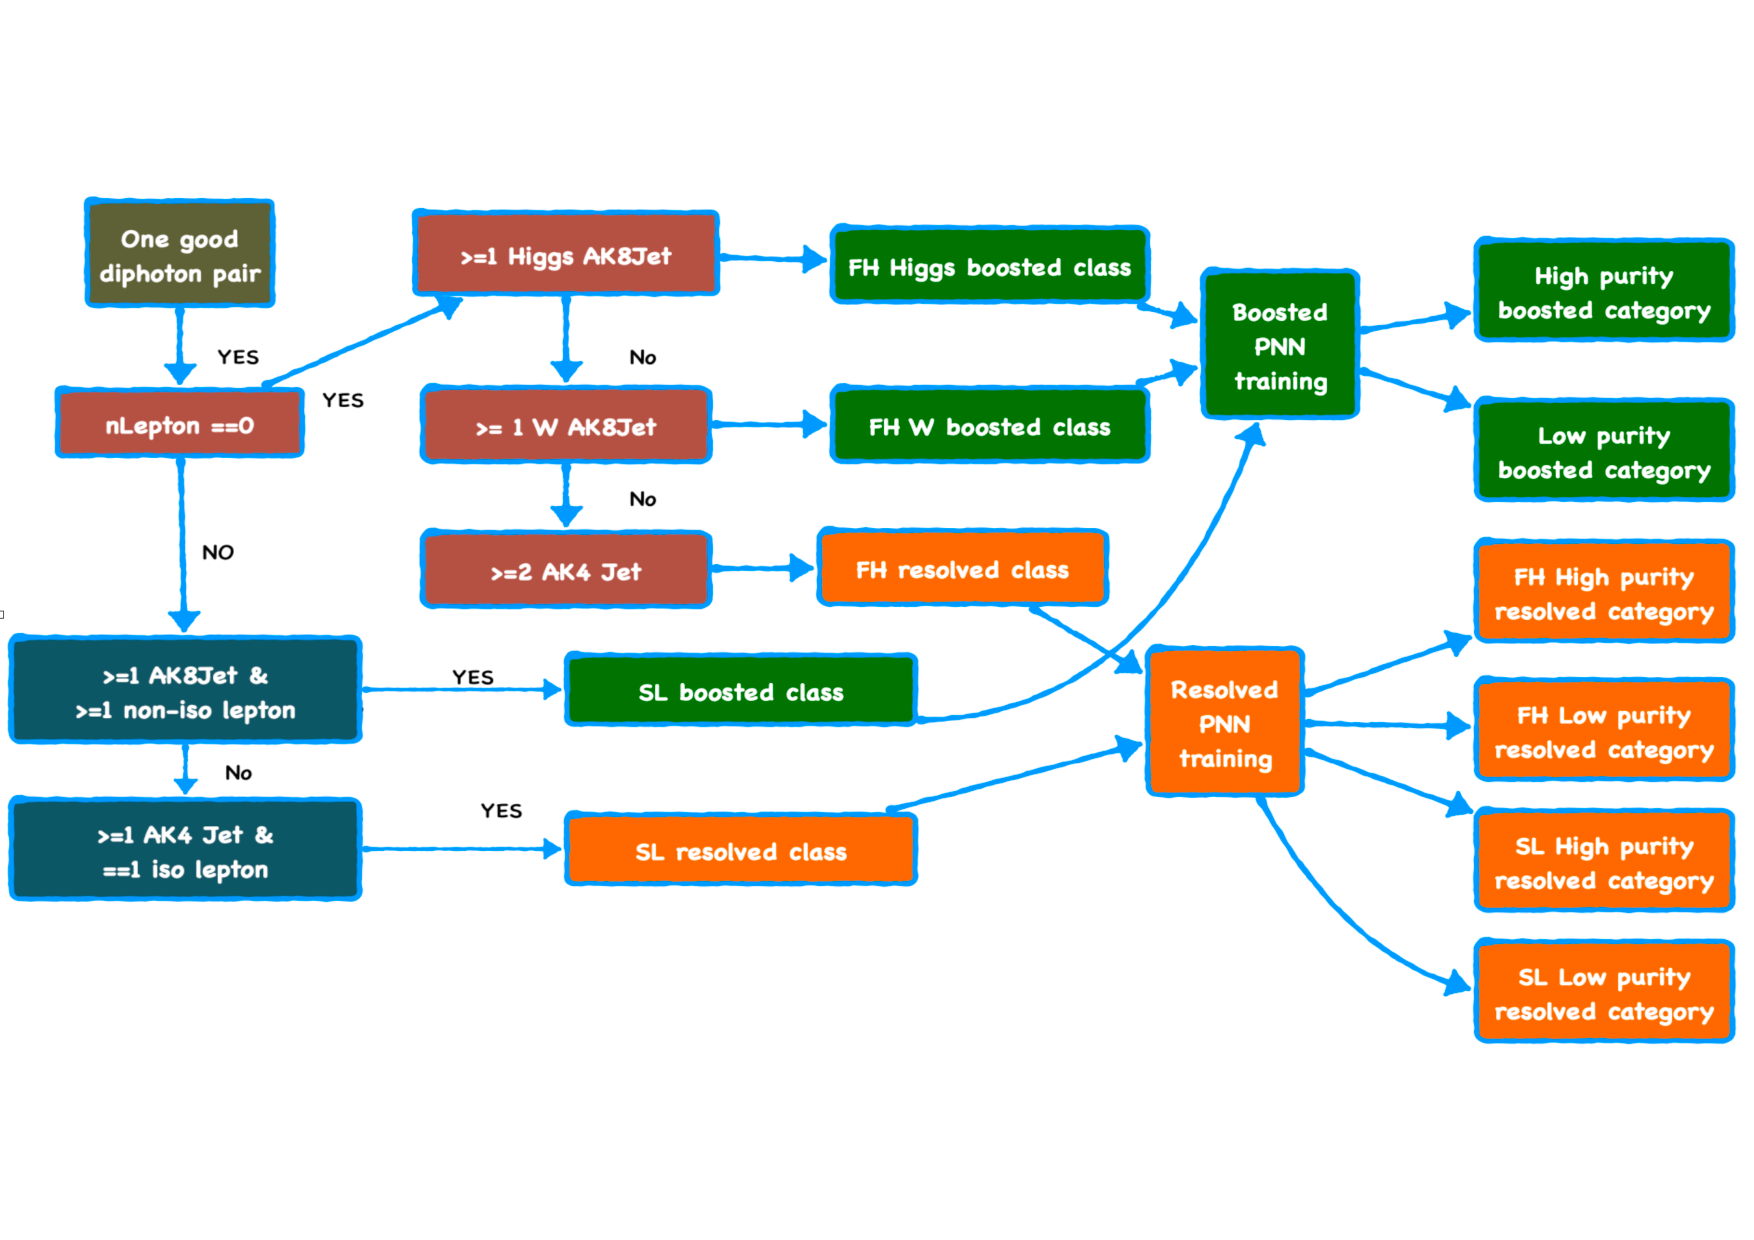
\includegraphics[width=0.95\textwidth]{figures/diHiggsSearches/EventSelectionWorkflow.pdf}
    \caption{Event selection workflow for the \HHWW analysis.}
    \label{fig:event_selection_workflow}
\end{figure}


\section{Data-Driven Background Estimation}
Accurately estimating background processes is crucial for isolating the \HHWW signal.
The dominant backgrounds include non-resonant diphoton production, single Higgs processes, and multijet events
where fake photons mimic the signal.
A data-driven approach is used to estimate fake photon contributions~\cite{CMS:2020cga}.

\subsection{Motivation}
The limited statistics of QCD Monte Carlo (MC) samples lead to poor modeling of key input features for multivariate analyses.
To ensure reliable machine learning training and data-MC agreement, a data-driven method is adopted~\cite{CMS:2020cga}.
This approach uses events from the photon ID MVA sideband to model fake photon contributions.

\subsection{Methodology}
The data-driven background estimation follows these steps:
\begin{enumerate}
    \item \textbf{Photon ID Sideband Selection:}
    Events failing the photon ID MVA preselection cut are used to model fake photons.
    The sideband regions are defined as:
    \begin{itemize}
        \item Resolved category: Photon ID MVA in \([-0.9, -0.7]\).
        \item Boosted category: Photon ID MVA in \([-0.95, -0.9]\).
    \end{itemize}

    \item \textbf{PDF Generation for Fake Photons:}
    A probability density function (PDF) for the photon ID MVA distribution of fake photons is
    derived from MC samples (e.g., \(\gamma + \text{jets}\)).
    Sideband events are reweighted to match the PDF in the signal region.

    \item \textbf{Reweighting and Normalization:}
    Per-event weights are applied to sideband events to reshape the photon ID MVA distribution.
    The weight \(w\) is defined as:
    \[
        w = \frac{\int_{\text{minID}}^{\text{maxID}} \text{fakePDF}(x) \, dx}
                 {\int_{\text{sidebandMinID}}^{\text{sidebandMaxID}} \text{fakePDF}(x) \, dx}.
    \]
    Separate weights are applied for resolved and boosted categories.

    \item \textbf{Validation:}
    The reweighted MC is normalized to data, and comparisons before and after reweighting show improved agreement in key variables like \(m_{\gamma\gamma}\).
\end{enumerate}

\subsection{Challenges and Solutions}
Despite its success, this method presents some challenges:
\begin{itemize}
    \item \textbf{Muon Channel in Semi-Leptonic (SL) Events:}
    While the method improves agreement in the electron channel, it worsens the muon channel.
    Potential solutions include:
    \begin{itemize}
        \item Applying the data-driven approach only to the electron channel.
        \item Using separate reweighting for electron and muon channels.
    \end{itemize}
    For now, we are using the additional MVA reweighting on top of this method to improve the overall agreement. As we don't use the MC for the signal extraction, the impact of this method on the signal extraction is minimal.

    \item \textbf{Photon ID Sidebands:}
    Key assumptions in this method include:
    \begin{enumerate}
        \item Photon ID MVA has minimal correlation with other analysis variables.
        \item The sideband is dominated by fake photons (e.g., QCD and \(\gamma + \text{jets}\)).
        \item Sideband photons are assumed to be entirely fake.
    \end{enumerate}
\end{itemize}

\subsection{Implementation in Different Channels}
The method is applied to both fully hadronic (FH) and semi-leptonic (SL) channels:
\begin{itemize}
    \item \textbf{Fully Hadronic Channel:}
    Dominated by QCD backgrounds, with the photon ID sideband effectively modeling fake photon contributions.
    \item \textbf{Semi-Leptonic Channel:}
    Includes contributions from \(W\gamma\gamma\) and \(t\bar{t}\) processes, with non-isolated leptons playing a key role in background estimation.
\end{itemize}

\subsection{Impact of the Data-Driven Method}
The data-driven background estimation significantly improves the analysis:
\begin{itemize}
    \item Enhanced modeling of photon-related variables in resolved and boosted categories.
    \item Improved agreement between data and MC in control regions, as shown in Fig.~\ref{fig:control_plots}.
        \begin{figure}[!htbp]
            \centering
            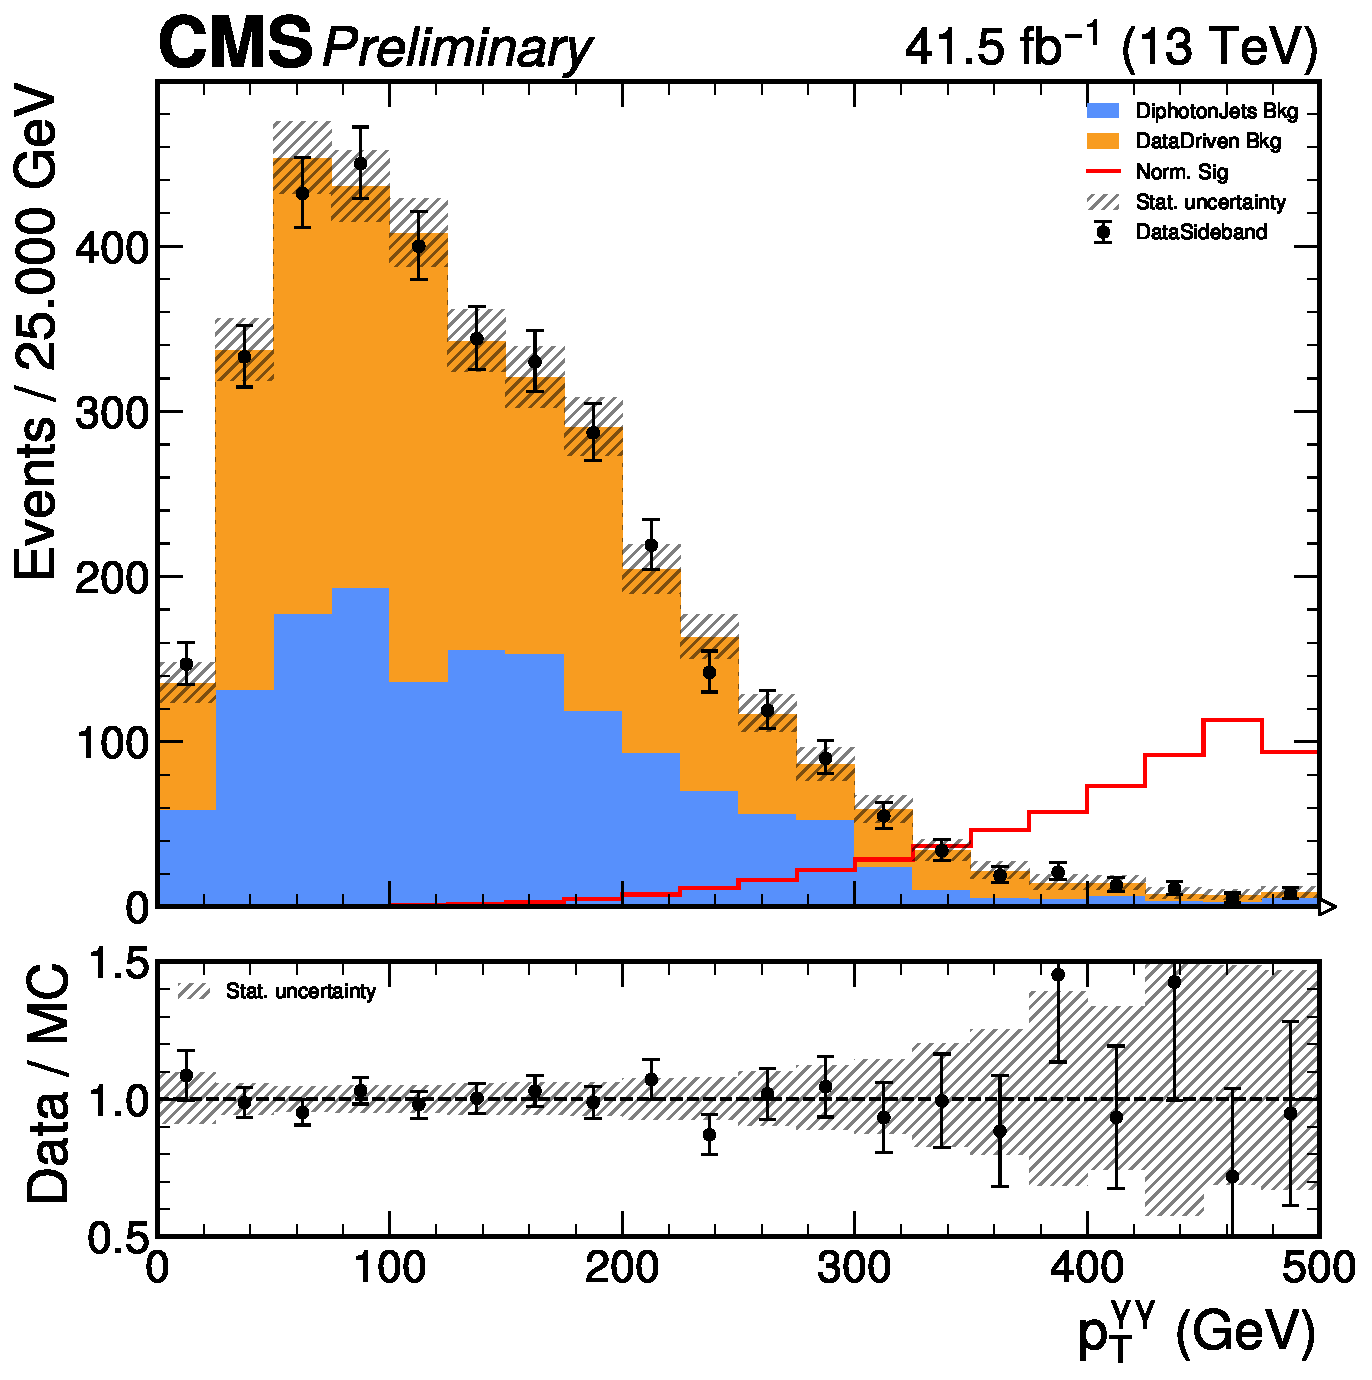
\includegraphics[width=0.45\textwidth]{figures/ControlPlots/boosted_PNN_reweighted/PNN_Diphoton_pt_after_reweight.pdf}%
            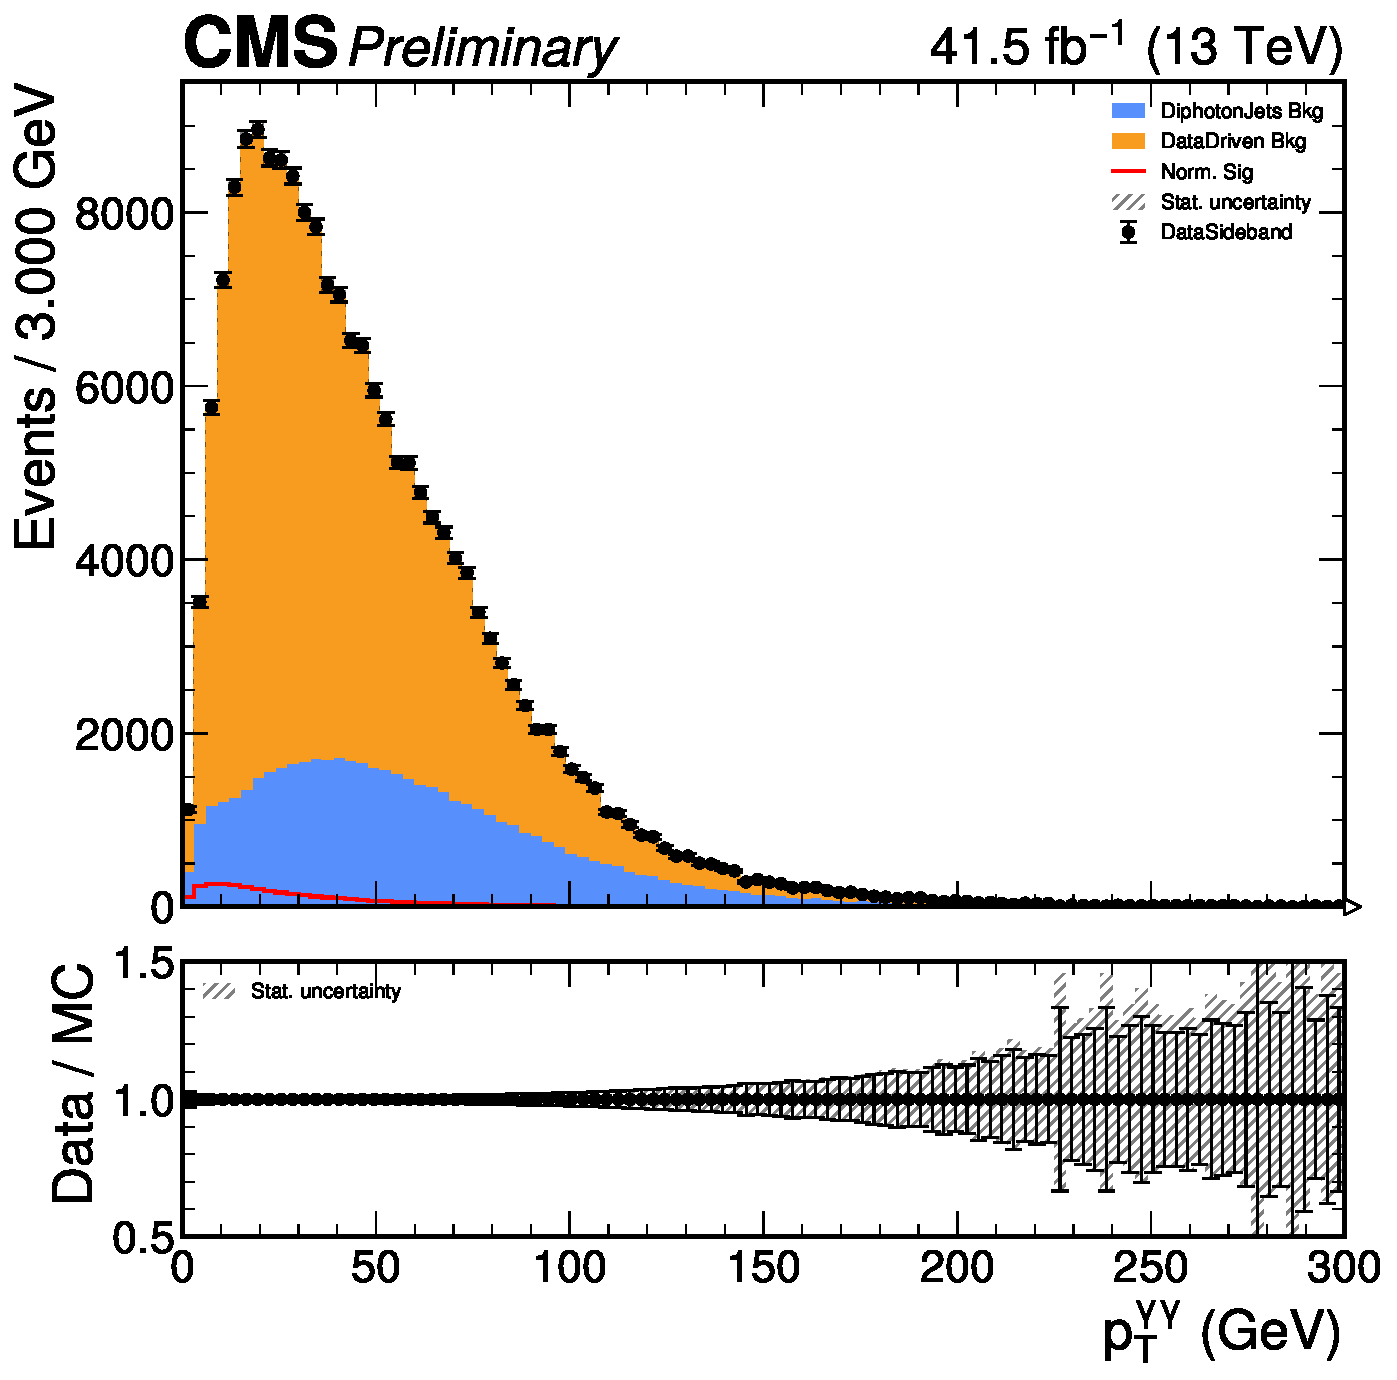
\includegraphics[width=0.45\textwidth]{figures/ControlPlots/resolved_PNN_reweighted/PNN_Diphoton_pt.pdf}
            \caption{Control plots showing the agreement between data and MC after applying the data-driven method. Left: Boosted category. Right: Resolved category.}
            \label{fig:control_plots}
        \end{figure}
\end{itemize}

\section{Multivariate Analysis Using Parameterized Neural Network (pNN)}
To maximize the sensitivity of the search for resonant \HHWW, a multivariate analysis (MVA) is performed
using a Parameterized Neural Network (pNN). The pNN method allows for simultaneous training across multiple signal hypotheses,
parameterized by the mass of the heavy resonance \(m_X\). This approach ensures a robust discrimination between signal and
background across a wide range of masses, from 250~GeV to 3000~GeV.

The pNN is implemented as a deep feed-forward neural network. Its inputs include kinematic and topological features of the events, with the resonance mass \(m_X\) incorporated as a parameter to generalize across different signal hypotheses. The network is trained using the Adam optimizer with stochastic gradient descent, and GPU acceleration is used for efficient processing of large datasets. Additional features, such as dropout layers, are included to prevent overfitting and enhance model generalization.

Separate pNNs are trained for the boosted and resolved topologies to account for the distinct event kinematics in these categories.
The boosted category includes events where \(W\)-bosons' decay products are merged into single AK8 jets, while the resolved category reconstructs \(W\)-bosons' decay products as individual AK4 jets.
Input features, such as photon, jet, and missing transverse energy (\(E_T^{\text{miss}}\)) observables, are carefully selected based on their ability to discriminate signal from background. These features include variables like the diphoton \(p_T/m_{\gamma\gamma}\), the angular separation (\(dR\)) between photons, and jet kinematics. The full list of input variables used for the boosted pNN training is provided in Table~\ref{tab:inputvariables_boosted} and for the resolved pNN training in Table~\ref{tab:inputvariables_resolved}.
\begin{table}[htbp!]
    \centering
    \begin{tabularx}{\textwidth}{|l|X|}
    \hline
    \textbf{Feature} & \textbf{Description} \\
    \hline
    Diphoton\_pTom & Transverse momentum of the diphoton system over the mass of the diphoton system \\
    Diphoton\_dR & Delta R between the two photons \\
    Diphoton\_eta & Pseudorapidity of the diphoton system \\
    Diphoton\_phi & Azimuthal angle of the diphoton system \\
    LeadPhoton\_pTom & Transverse momentum of the leading photon over the mass of the diphoton system \\
    SubleadPhoton\_pTom & Transverse momentum of the subleading photon over the mass of the diphoton system \\
    LeadPhoton\_eta & Pseudorapidity of the leading photon \\
    LeadPhoton\_phi & Azimuthal angle of the leading photon \\
    SubleadPhoton\_eta & Pseudorapidity of the subleading photon \\
    SubleadPhoton\_phi & Azimuthal angle of the subleading photon \\
    fatjet\_1\_pT & Transverse momentum of the leading fatjet \\
    fatjet\_1\_eta & Pseudorapidity of the leading fatjet \\
    fatjet\_1\_phi & Azimuthal angle of the leading fatjet \\
    fatjet\_1\_mass & Mass of the leading fatjet \\
    fatjet\_2\_pT & Transverse momentum of the subleading fatjet \\
    fatjet\_2\_eta & Pseudorapidity of the subleading fatjet \\
    fatjet\_2\_phi & Azimuthal angle of the subleading fatjet \\
    fatjet\_2\_mass & Mass of the subleading fatjet \\
    fatjet\_1\_2\_dR & Delta R between the two fatjets \\
    fatjet\_1\_diphoton\_dR & Delta R between the leading fatjet and the diphoton system \\
    fatjet\_2\_diphoton\_dR & Delta R between the subleading fatjet and the diphoton system \\
    fatjet\_1\_leadphoton\_dR & Delta R between the leading fatjet and the leading photon \\
    fatjet\_1\_subleadphoton\_dR & Delta R between the leading fatjet and the subleading photon \\
    fatjet\_2\_leadphoton\_dR & Delta R between the subleading fatjet and the leading photon \\
    fatjet\_2\_subleadphoton\_dR & Delta R between the subleading fatjet and the subleading photon \\
    max\_fatjets\_mass & Maximum mass of the two fatjets \\
    nGoodAK4jets & Number of good AK4 jets \\
    nGoodAK8jets & Number of good AK8 jets \\
    Third leading jets\_pT & Transverse momentum of the third leading jets \\
    Third leading jets\_eta & Pseudorapidity of the third leading jets \\
    Third leading jets\_phi & Azimuthal angle of the third leading jets \\
    Third leading jets\_mass & Mass of the third leading jets \\
    PuppiMET\_pt & Transverse momentum of the missing transverse energy \\
    dphi\_jet1\_PuppiMET & Azimuthal angle difference between the first jet and missing transverse energy \\
    dphi\_jet2\_PuppiMET & Azimuthal angle difference between the second jet and missing transverse energy \\
    PuppiMET\_sumEt & Sum of the transverse energy of the missing transverse energy \\
    MX & Invariant mass of the resonance X \\
    \hline
    \end{tabularx}
    \caption{Input variables used for the boosted PNN training.}
    \label{tab:inputvariables_boosted}
\end{table}
\begin{table}[htbp!]
    \centering
    \begin{tabularx}{\textwidth}{|l|X|}
    \hline
    \textbf{Feature} & \textbf{Description} \\
    \hline
    MX & Invariant mass of the resonance X \\
    Diphoton\_pTom & Transverse momentum of the diphoton system over the mass of the diphoton system \\
    Diphoton\_eta & Pseudorapidity of the diphoton system \\
    Diphoton\_phi & Azimuthal angle of the diphoton system \\
    LeadPhoton\_pTom & Transverse momentum of the leading photon over the mass of the diphoton system \\
    SubleadPhoton\_pTom & Transverse momentum of the subleading photon over the mass of the diphoton system \\
    LeadPhoton\_eta & Pseudorapidity of the leading photon \\
    LeadPhoton\_phi & Azimuthal angle of the leading photon \\
    SubleadPhoton\_eta & Pseudorapidity of the subleading photon \\
    SubleadPhoton\_phi & Azimuthal angle of the subleading photon \\
    Diphoton\_dR & Delta R between the two photons \\
    Diphoton\_dEta & Delta pseudorapidity between the two photons \\
    jet\_1\_2\_pt & Transverse momentum of the combined leading and subleading jets \\
    jet\_1\_2\_mass & Mass of the combined leading and subleading jets \\
    jet\_1\_2\_dR & Delta R between the leading and subleading jets \\
    jet\_1\_pt & Transverse momentum of the leading jet \\
    jet\_2\_pt & Transverse momentum of the subleading jet \\
    photon1\_jet1\_dR & Delta R between the leading photon and the leading jet \\
    photon1\_jet2\_dR & Delta R between the leading photon and the subleading jet \\
    photon1\_jet1\_2\_dR & Delta R between the leading photon and the combined leading and subleading jets \\
    Diphoton\_jet1\_2\_dR & Delta R between the diphoton system and the combined leading and subleading jets \\
    Diphoton\_jet1\_dR & Delta R between the diphoton system and the leading jet \\
    Diphoton\_jet2\_dR & Delta R between the diphoton system and the subleading jet \\
    photon2\_jet1\_dR & Delta R between the subleading photon and the leading jet \\
    photon2\_jet2\_dR & Delta R between the subleading photon and the subleading jet \\
    photon2\_jet1\_2\_dR & Delta R between the subleading photon and the combined leading and subleading jets \\
    Diphoton\_jet\_1\_2\_dEta & Delta pseudorapidity between the diphoton system and the combined leading and subleading jets \\
    Diphoton\_jet\_1\_dEta & Delta pseudorapidity between the diphoton system and the leading jet \\
    Diphoton\_jet\_2\_dEta & Delta pseudorapidity between the diphoton system and the subleading jet \\
    Diphoton\_jet\_1\_2\_dPhi & Delta phi between the diphoton system and the combined leading and subleading jets \\
    Diphoton\_jet\_1\_dPhi & Delta phi between the diphoton system and the leading jet \\
    Diphoton\_jet\_2\_dPhi & Delta phi between the diphoton system and the subleading jet \\
    PuppiMET\_pt & Transverse momentum of the missing transverse energy \\
    nGoodAK4jets & Number of good AK4 jets \\
    nGoodisoleptons & Number of good isolated leptons \\
    leading\_bscore & B-tagging score of the leading jet \\
    subleading\_bscore & B-tagging score of the subleading jet \\
    sum\_two\_max\_bscores & Sum of the two highest b-tagging scores \\

    \hline
    \end{tabularx}
    \caption{Input variables used for the resolved PNN training.}
    \label{tab:inputvariables_resolved}
\end{table}

The performance of the pNN is evaluated using metrics such as the area under the curve (AUC) and signal-to-background ratio improvements. The pNN demonstrates significant enhancement in discrimination between signal and background across the entire mass range. Feature importance plots highlight the critical role of variables such as diphoton \(p_T/m_{\gamma\gamma}\) and photon angular separations in improving sensitivity. Separate training for the boosted and resolved categories further optimizes the analysis for these topologies.

The output of the pNN serves as the final discriminant for signal extraction in the \(m_{\gamma\gamma}\) distribution. By combining the boosted and resolved categories, the analysis achieves a 60\% improvement in sensitivity compared to previous results. Control plots of key variables before and after applying the pNN show excellent agreement between data and Monte Carlo, validating the robustness of the method.

The parameterized neural network approach thus provides a powerful framework for signal extraction in the \HHWW analysis. By training across multiple mass hypotheses and incorporating advanced multivariate techniques, the pNN significantly improves the sensitivity to resonant di-Higgs production, particularly in high-mass regions.



\section{Summary and Outlook}
This analysis represents the first CMS study of resonant di-Higgs production in the \(WW\gamma\gamma\) channel, covering all possible jet topologies and using advanced machine learning techniques like parameterized neural networks. The results provide significant constraints on BSM scenarios predicting heavy resonances decaying into Higgs boson pairs.

Future plans include:
\begin{itemize}
    \item Extending the analysis to include non-resonant di-Higgs production.
    \item Finalizing results for publication with a target timeline of Moriond 2025.
\end{itemize}
